\section{Fault localization}

%% what are the claims, what are we studying, why are we studying it

\subsection{Coverage}

\rqorinsight{RQ2: Do failing tests cover different portions of the fault?}

SBFL is the most commonly used, as well as the most 
effective~\cite{zou2019empirical}, fault localization technique. As a result, 
it serves as an important first step in narrowing down the search 
space for program repair.

The assumption underlying SBFL is that failing tests execute buggy portions of 
the code more often than passing tests. Thus, if all failing tests execute a 
particular line of code, then that line of code is scored as more suspicious. 
However, if the failing tests cover different portions of the buggy code, then 
this assumption no longer holds, and SBFL would lose effectiveness.

Therefore, for multi-edit bugs with multiple identifying failing tests, do the 
different failing tests cover exactly the same patch locations, exactly 
disjoint path locations, or some combination?

\paragraph{Methodology}

Between both datasets, there are 60 total bugs that are both multi-edit and 
multi-test -- 45 in Defects4J and 15 in Bears. For each of these bugs, we used 
Jacoco to determine which of the chunks in the human patch were executed by each failing test. Using 
this coverage data, we categorized the bug as one of 
three coverage patterns: \textit{disjoint} for bugs in which no chunk is covered by all failing tests, 
\textit{same} for bugs in which all 
tests cover the exact same chunks of the patch, and \textit{overlap} for all 
other bugs, where some chunks are covered by all failing tests, but some chunks are only covered by a 
subset of failing tests.

\paragraph{Results}
The overall distribution is seen in Figure \ref{fig:coverage-all}. Over a third 
of the bugs were classified as disjoint, indicating that for a significant 
portion of bugs, the failing tests do not all execute any portion of the faulty 
code. In addition, another 22\% were classified as overlap. Thus, over half of 
the bugs that were both multi-edit and multi-test contained chunks that were 
not executed by all failing test cases.
2

\begin{figure}
	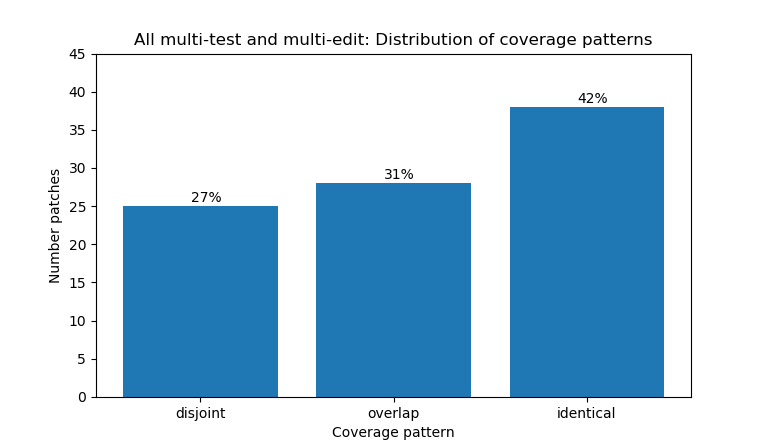
\includegraphics[width=\linewidth]{img/coverage-all.png}
	\caption{Distribution of coverage patterns for all multi-test and 
	multi-edit bugs in Bears and Defects4J. In all, 38\% of bugs were classified as disjoint, 40\% were 
	classified as same, and 22\% were classified as overlap.}
	\label{fig:coverage-all}
\end{figure}

SBFL assumes that faulty locations are executed more often by identifying 
or failing test cases and is not designed to find faults like these. Since SBFL 
is the most common fault localization technique in APR, most APR techniques 
are not well suited to fix a majority of these multi-edit and multi-test 
bugs.

If we divide distribution by dataset, we can see even more interesting 
behavior. Figure \ref{fig:coverage-datasets} shows the Defects4J dataset and 
the Bears dataset have very different distributions with respect to the 
disjoint and same categories -- in Defects4J, 47\% of bugs are disjoint and 
31\% are same, whereas in Bears, the proportions are 13\% disjoint and 67\% 
same. We hypothesize that this may be due to differences in how the two 
datasets were minimized, since Defects4J is a dataset of minimized and curated 
bugs while the bugs in Bears are taken scraped directly from the commits.


\begin{figure}
	\begin{subfigure}{\linewidth}
		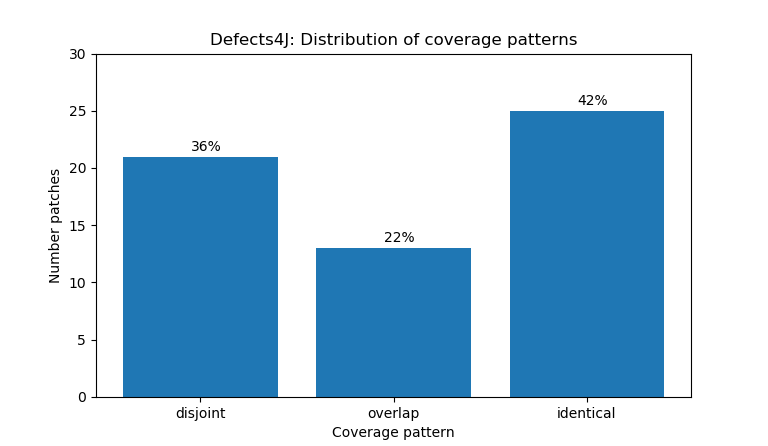
\includegraphics[width=\linewidth]{img/coverage-d4j.png}
		\caption{Distribution of coverage patterns for Defects4J. 47\% disjoint, 31\% same, and 22\% 
		overlap.}
	\end{subfigure}
	\begin{subfigure}{\linewidth}
		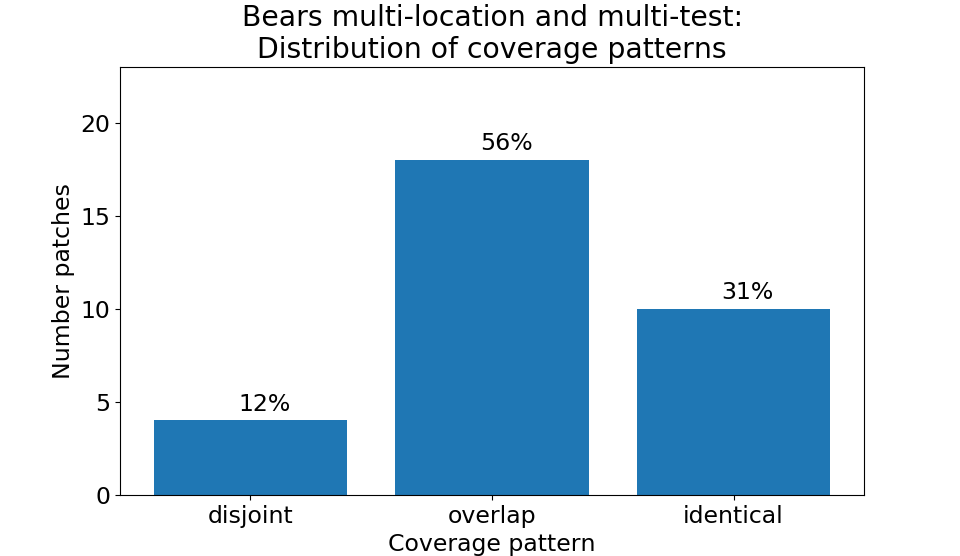
\includegraphics[width=\linewidth]{img/coverage-bears.png}
		\caption{Distribution of coverage patterns for Defects4J. 13\% disjoint, 67\% same, and 20\% 
		overlap.}
	\end{subfigure}
	\caption{Distribution of coverage patterns divided by dataset.}
	\label{fig:coverage-datasets}
\end{figure}


\section{Symptoms}

We want to study symptoms in the context of fault localization. We define symptoms as the output given in failing test cases. In Java, most of these symptoms will be exceptions and their accompanying error message. Since most program repair is based off of failing tests, we want to see if those symptoms exhibited in those tests can correlate to type of repair.

For this paper, we specifically wanted to look at whether symptoms correlated with whether a bug could be fixed in a single location or multiple locations. If we can classify which bugs are single edit or multi edit, we can choose fault localization or patch generation techniques that are more suited.

We looked at all symptoms for all bugs in Defects4J and Bears, and categorized them based on whether they were one of the identified multi-chunk bugs or not. Then we fit the data to a linear regression model to see if there were statistically significant differences between the type of symptoms for multi edit and single edit bugs.

In order to find statistical significance, we needed to categorize the symptoms in big enough categories. We experimented with three groupings:

\begin{enumerate}
	\item Group all exceptions together except for assertion exceptions and exceptions for which a message indicates some sort of assertion (in our case, we simply looked for the keyword "expected"). We grouped the assertions into a few different types: 
	\begin{itemize}
		\item \lstinline{assert_null} is when the assertion is either expecting null, or got null when it wasn't expecting it.
		\item \lstinline{assert_int} is when the failing assertion was expecting a particular int value.
		\item \lstinline{assert_float} is the same as above, but for floats.
		\item \lstinline{assert_obj_arr_date} is when the assertion is expecting an object address, array of objects, or date object/date string. These are grouped together as commonly found but more complex assertions.
		\item \lstinline{error_expected} is when the failing test expected an exception, error, or warning.
		\item \lstinline{timeout} is when a Junit test times out, but also includes errors like stack overflows or out of memory exceptions.
		\item \lstinline{other_assert} for any other assertion that I couldn't easily categorize or parse. The large bulk of bugs in this category are bugs that had no error message at all; it simply failed with an \lstinline{AssertionError} or \lstinline{StackOverflow}.
		\item \lstinline{other}: all non-assertion exceptions.
	\end{itemize}
	\item Grouping symptoms together in an ad hoc way \todo{sell it better.}
	\begin{itemize}
		\item \lstinline{assert_prim}: assertions that compare to a Java primitive, such as int, float, or boolean.
		\item \lstinline{assert_null}: either expected or actual is null
		\item \lstinline{other_assert}: Asserting to anything that's not clearly a primitive or null.
		\item \lstinline{access}: all the bugs pertaining to wrongfully accessing or invoking certain fields or methods, or problems with classpath.
		\item \lstinline{null_pointer}: null pointer exceptions.
		\item \lstinline{timeout}: when a Junit test times out, but also includes errors like stack overflows or out of memory exceptions.
		\item \lstinline{parsing}: Anything related to parsing, serialization, or type conversion.
		\item \lstinline{other}: everything else
	\end{itemize}
	\item This last grouping is an even coarser version of the previous grouping.
	\begin{itemize}
		\item \lstinline{assert_equal}: Any assertion in which the test expected one value but got another
		\item \lstinline{other_assert}: any other assertion
		\item \lstinline{access}: all the bugs pertaining to wrongfully accessing or invoking certain fields or methods, or problems with classpath.
		\item \lstinline{null_pointer}: null pointer exceptions.
		\item \lstinline{parsing}: Anything related to parsing, serialization, or type conversion.
		\item \lstinline{other}: everything else
	\end{itemize}
\end{enumerate}

\todo{raw data from bogdan:}

assert only
\begin{lstlisting}
Call:
glm(formula = multi ~ assert_obj_arr_date + assert_int + assert_float + 
error_expected + timeout + assert_null + other_assert + other, 
family = "binomial", data = symptoms)Deviance Residuals: 
Min       1Q   Median       3Q      Max  
-1.2466  -0.5686  -0.4691  -0.4394   2.2880  Coefficients:
Estimate Std. Error z value Pr(>|z|)    
(Intercept)             -2.37550    0.38061  -6.241 4.34e-10 ***
assert_obj_arr_dateTRUE  1.24082    0.50907   2.437   0.0148 *  
assert_intTRUE           0.08619    0.45621   0.189   0.8502    
assert_floatTRUE         2.31273    0.48580   4.761 1.93e-06 ***
error_expectedTRUE       0.36735    0.53943   0.681   0.4959    
timeoutTRUE              0.99295    0.65378   1.519   0.1288    
assert_nullTRUE         -0.16611    0.58071  -0.286   0.7748    
other_assertTRUE         0.22402    0.36136   0.620   0.5353    
otherTRUE                0.63507    0.38201   1.662   0.0964 .  
---
Signif. codes:  0 '***' 0.001 '**' 0.01 '*' 0.05 '.' 0.1 ‘ ’ 1(Dispersion parameter for binomial family taken to be 1)    Null deviance: 546.49  on 645  degrees of freedom
Residual deviance: 510.11  on 637  degrees of freedom
AIC: 528.11Number of Fisher Scoring iterations: 5
\end{lstlisting}

grouping 1
\begin{lstlisting}
Call:
glm(formula = multi ~ access + assert_prim + null_pointer + timeout + 
assert_null + parsing + other_assert + other, family = "binomial", 
data = symptoms)Deviance Residuals: 
Min       1Q   Median       3Q      Max  
-0.9771  -0.6792  -0.5070  -0.4031   2.5944  Coefficients:
Estimate Std. Error z value Pr(>|z|)    
(Intercept)      -1.94778    0.36198  -5.381 7.41e-08 ***
accessTRUE        0.62756    0.41197   1.523   0.1277    
assert_primTRUE   0.81567    0.36223   2.252   0.0243 *  
null_pointerTRUE  0.32833    0.52496   0.625   0.5317    
timeoutTRUE       0.64782    0.63743   1.016   0.3095    
assert_nullTRUE  -0.52160    0.57971  -0.900   0.3682    
parsingTRUE       0.64081    0.50451   1.270   0.2040    
other_assertTRUE -0.03905    0.34777  -0.112   0.9106    
otherTRUE        -1.38263    0.76326  -1.811   0.0701 .  
---
Signif. codes:  0 '***' 0.001 '**' 0.01 '*' 0.05 '.' 0.1 ‘ ’ 1(Dispersion parameter for binomial family taken to be 1)    Null deviance: 546.49  on 645  degrees of freedom
Residual deviance: 523.84  on 637  degrees of freedom
AIC: 541.84Number of Fisher Scoring iterations: 5
\end{lstlisting}

grouping 2
\begin{lstlisting}
Call:
glm(formula = multi ~ assert_equal + access + null_pointer + 
parsing + other_assert + other, family = "binomial", data = symptoms)Deviance Residuals: 
Min       1Q   Median       3Q      Max  
-0.9390  -0.6809  -0.4377  -0.4377   2.2494  Coefficients:
Estimate Std. Error z value Pr(>|z|)    
(Intercept)       -2.0821     0.3470  -6.001 1.96e-09 ***
assert_equalTRUE   0.7532     0.3333   2.260   0.0238 *  
accessTRUE         0.7259     0.3979   1.824   0.0681 .  
null_pointerTRUE   0.4338     0.5131   0.845   0.3979    
parsingTRUE        0.7385     0.4976   1.484   0.1378    
other_assertTRUE  -0.2150     0.3223  -0.667   0.5048    
otherTRUE         -0.3646     0.5068  -0.719   0.4719    
---
Signif. codes:  0 '***' 0.001 '**' 0.01 '*' 0.05 '.' 0.1 ‘ ’ 1(Dispersion parameter for binomial family taken to be 1)    Null deviance: 546.49  on 645  degrees of freedom
Residual deviance: 527.48  on 639  degrees of freedom
AIC: 541.48Number of Fisher Scoring iterations: 5
\end{lstlisting}

In assert only, \lstinline{assert_float} correlates strongly with multiedit bugs. However, all the instances of \lstinline{assert_float} as a symptom occur in the Math package for Defects4J, and they all somehow to be multichunk. The sampling of \lstinline{assert_float} can be seenin the other two groupings as well, where \lstinline{asset_prim} and \lstinline{assert_equal}, both of which subsume \lstinline{assert_float}, are both more likey to be multi-edit.  \todo{take out math, redo analysis?}



\subsection{Discussion}
\todo{trying to elicit some takeaways here, not sure if this will stay in.}

We learned:
\begin{itemize}
	\item There are lots of multi-edit bugs in which no portion of the patch is covered by all failing 
	tests.
	\item However, there are also lots of multi-edit bugs that are covered exactly the same way by all 
	failing tests.
	\item Maybe next work includes what makes a disjoint bug disjoint; what makes a same patch 
	same? Correlate with symptoms? oooh.
	\item Speaking of symptoms, symptoms in the parsing category seems to correlate with 
	multi-chunk bugs as well as decreased repair success by existing APR tools, suggesting that ... 
	APR tools don't work well on multi-edit bugs?
\end{itemize}
